%==============================================================================
% CHAPTER 4 --- SYSTEM DESIGN
%==============================================================================

\chapter{System Design}
\label{chap:design}

\chapterquote{Good software architecture minimizes complexity while maximizing scalability, maintainability, and reliability.}{Martin Fowler}

%==============================================================================
\section{Overview}
\label{sec:design_overview}

This chapter presents the architectural design of the proposed NABTA platform. The system was designed following a modular and service-oriented architecture to facilitate scalability, maintainability, and seamless integration between multiple artificial intelligence models and cloud services.

The NABTA platform combines modern web technologies, deep learning, machine learning, explainable artificial intelligence, and cloud computing into a unified smart agriculture platform. The overall architecture separates the presentation layer, business logic, artificial intelligence services, and cloud infrastructure, allowing each subsystem to evolve independently while maintaining efficient communication through RESTful APIs.

The design focuses on four primary objectives:

\begin{itemize}
\item High-performance AI inference for real-time plant disease diagnosis.
\item Modular architecture that supports independent development and maintenance.
\item Secure communication between frontend, backend, and cloud services.
\item Scalable deployment capable of supporting multiple concurrent users.
\end{itemize}

The following sections describe the overall architecture, system workflow, UML diagrams, database design, API architecture, deployment strategy, and security mechanisms adopted in the implementation of the NABTA platform.

%==============================================================================
%==============================================================================
\section{System Workflow}
\label{sec:system_workflow}

The operational workflow of NABTA consists of a sequence of interconnected software modules that cooperate to provide intelligent agricultural services. Figure~\ref{fig:system_workflow} illustrates the overall execution flow of the platform.

\begin{figure}[H]
\centering
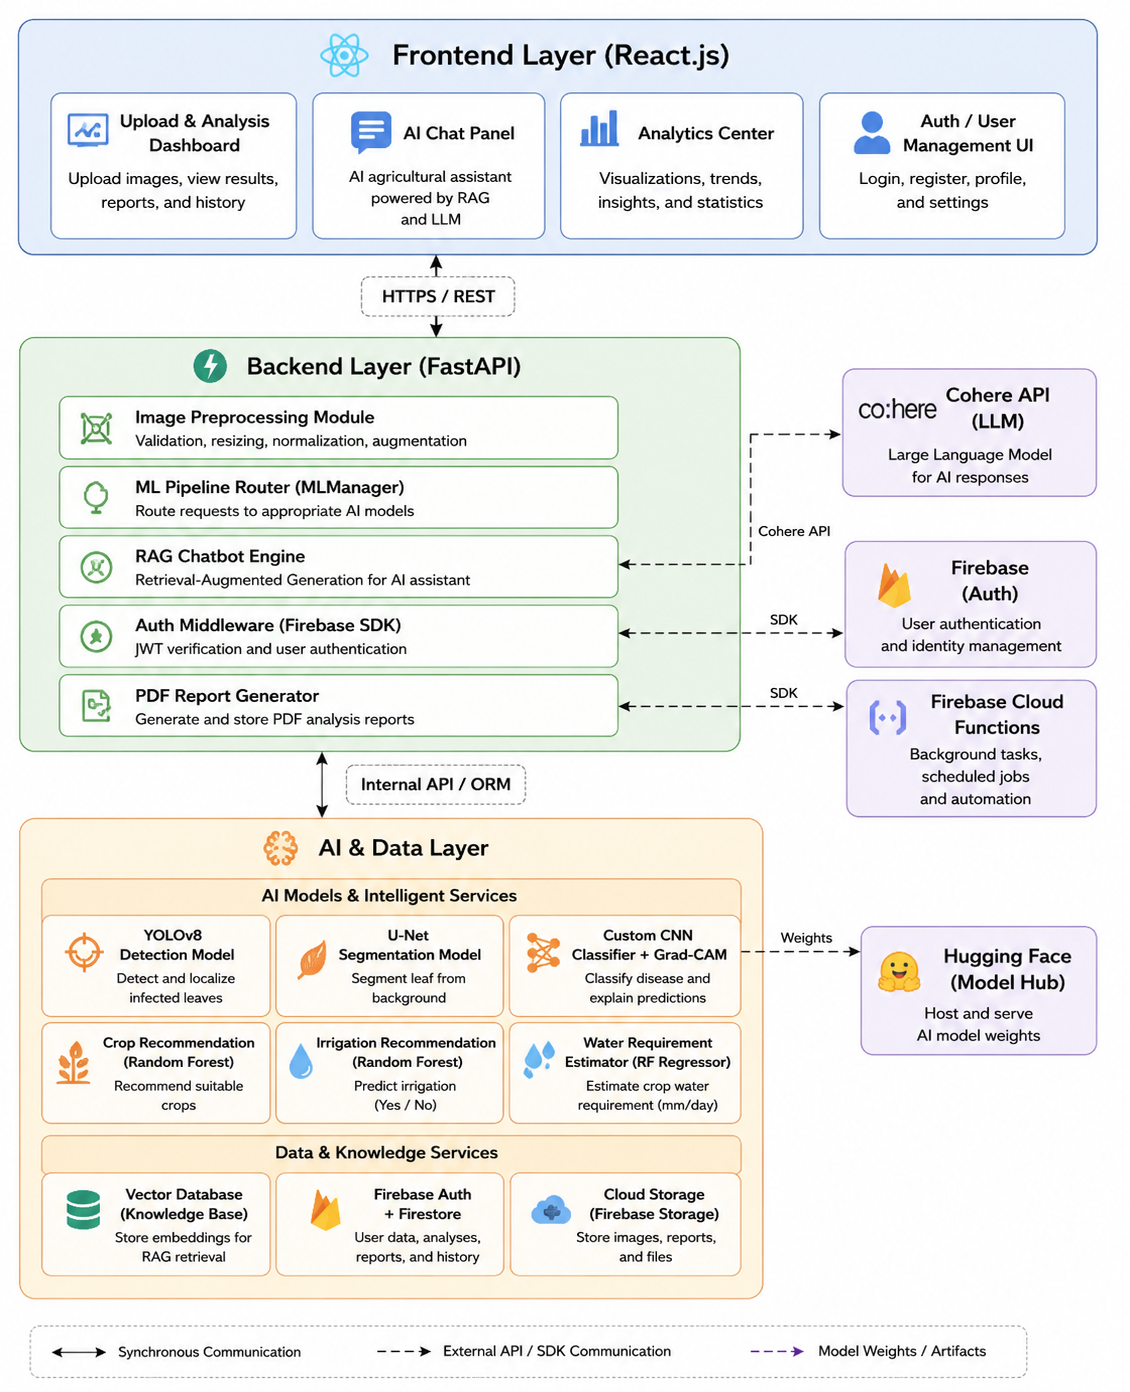
\includegraphics[width=\textwidth]{assets/diagrams/system_workflow.png}
\caption{Overall Workflow of the NABTA Platform}
\label{fig:system_workflow}
\end{figure}

The Presentation Layer consists of a React.js web application that provides users with interactive interfaces for plant disease analysis, irrigation prediction, crop recommendation, AI consultation, historical analysis, dashboard visualization, and account management.

The Application Layer is implemented using FastAPI, which acts as the central orchestration server. It manages user authentication, image preprocessing, request routing, communication with artificial intelligence models, report generation, database interaction, and external API integration.

The Artificial Intelligence Layer contains all deployed intelligent models used throughout the platform. These include the YOLOv8x object detector for infected leaf localization, the U-Net segmentation model with an EfficientNet-B0 encoder for leaf extraction, the custom CNN classifier for plant disease recognition, Grad-CAM for explainability and disease severity estimation, a Random Forest classifier for crop recommendation, a Random Forest classifier for irrigation decision prediction, and a Random Forest regressor for estimating crop water requirements.

The Cloud Data Layer integrates Firebase Authentication, Cloud Firestore, Firebase Cloud Functions, the Cohere API, Retrieval-Augmented Generation (RAG), and Hugging Face model hosting. These services collectively provide secure authentication, cloud data storage, conversational AI capabilities, document retrieval, and deployment of trained deep learning models.

This layered architecture enables loose coupling between software components, simplifies maintenance, improves scalability, and allows each subsystem to be updated independently without affecting the remaining parts of the platform.

%==============================================================================
\begin{figure}[H]
\centering
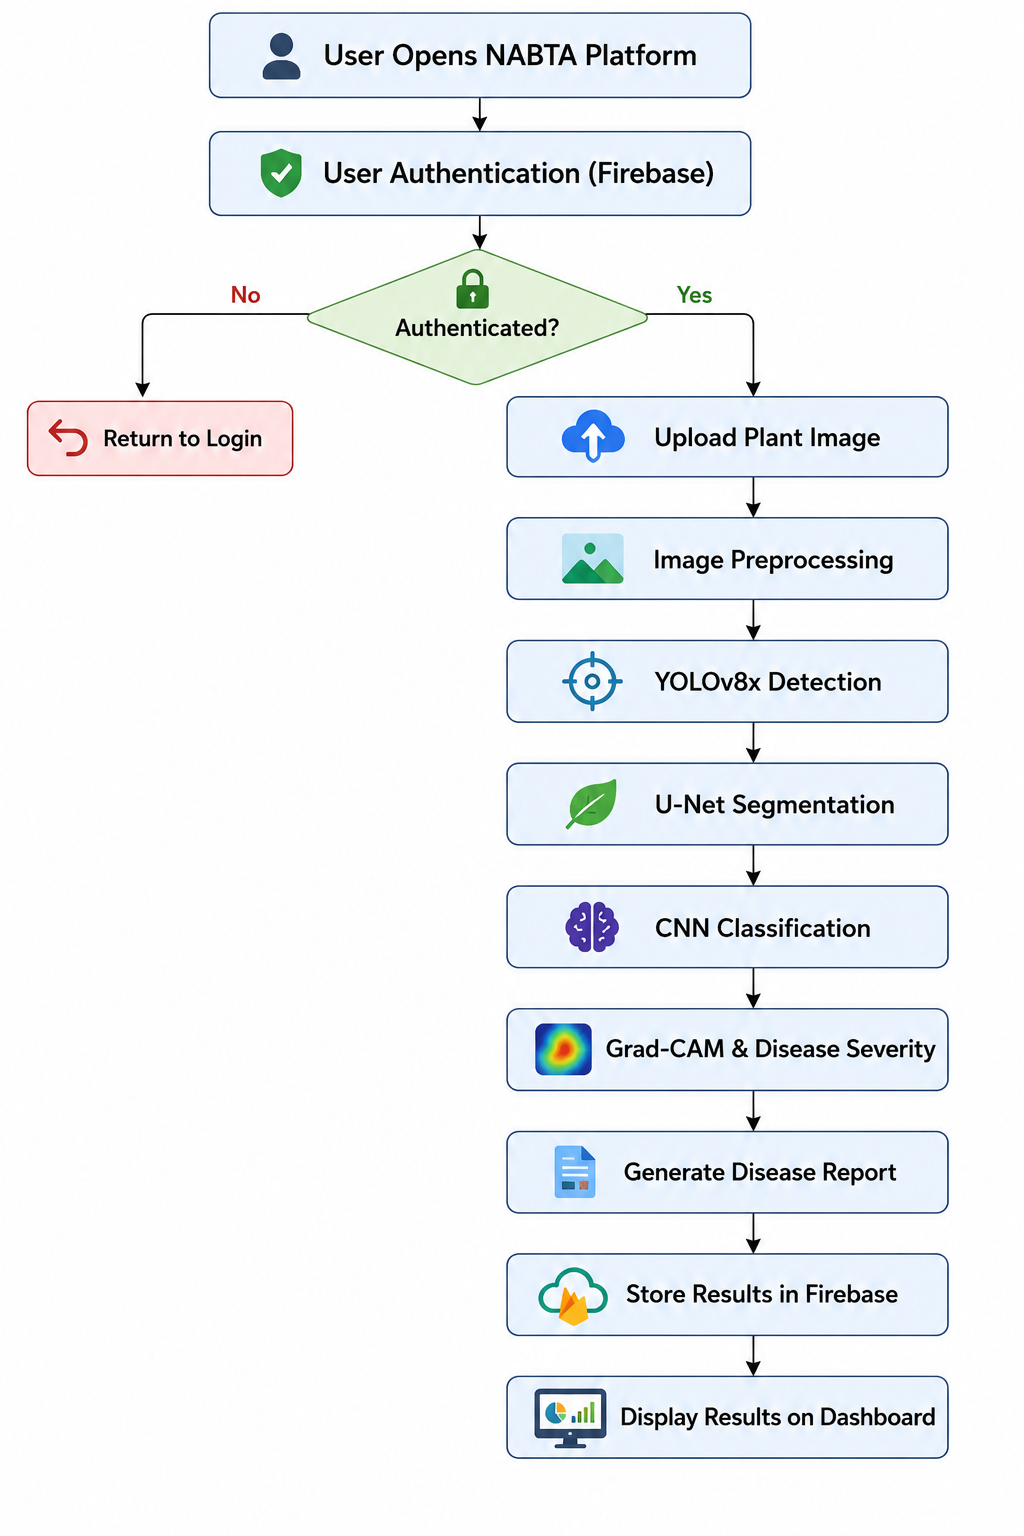
\includegraphics[width=0.85\textwidth]{assets/diagrams/system_workflows.png}
\caption{Overall Workflow of the NABTA Platform}
\label{fig:system_workflow}
\end{figure}

The execution process begins when a user accesses the web application through the React.js frontend. After successful authentication using Firebase Authentication, users can access the available intelligent services including plant disease analysis, crop recommendation, irrigation management, AI consultation, and historical records.

For plant disease diagnosis, the user uploads a leaf image through the Plant Analysis interface. The uploaded image is transmitted to the FastAPI backend, which performs image validation and preprocessing before initiating the artificial intelligence pipeline.

The AI pipeline executes four consecutive stages. First, the YOLOv8x model detects and localizes the infected leaf region. Second, the detected region is forwarded to the U-Net segmentation model, which separates the leaf from the surrounding background. Third, the segmented leaf image is analyzed by the custom CNN classifier to determine the plant species and disease category. Finally, Grad-CAM generates an explainability heatmap while simultaneously estimating disease severity based on the highlighted infected regions.

The generated results, including the detected disease, confidence score, segmentation mask, Grad-CAM visualization, and severity estimation, are stored in Cloud Firestore and displayed through the frontend interface. Users may also generate a PDF report containing the complete diagnosis.

The platform additionally provides two intelligent decision-support services. The crop recommendation module predicts the most suitable crops based on soil characteristics and environmental conditions, while the irrigation management module predicts irrigation requirements and estimates crop water demand using dedicated Random Forest models.

For agricultural consultation, user queries are processed through the Retrieval-Augmented Generation (RAG) pipeline. Relevant agricultural documents are first retrieved from the knowledge base before the query is forwarded to the Cohere Large Language Model, ensuring that generated responses remain domain-specific and evidence-based.

This workflow integrates multiple artificial intelligence techniques within a unified architecture while maintaining efficient communication between all system components.

%==============================================================================
\section{Use Case Diagram}
\label{sec:use_case}

The functional requirements of the NABTA platform are represented using the UML Use Case Diagram shown in Figure~\ref{fig:use_case}.

\begin{figure}[H]
\centering
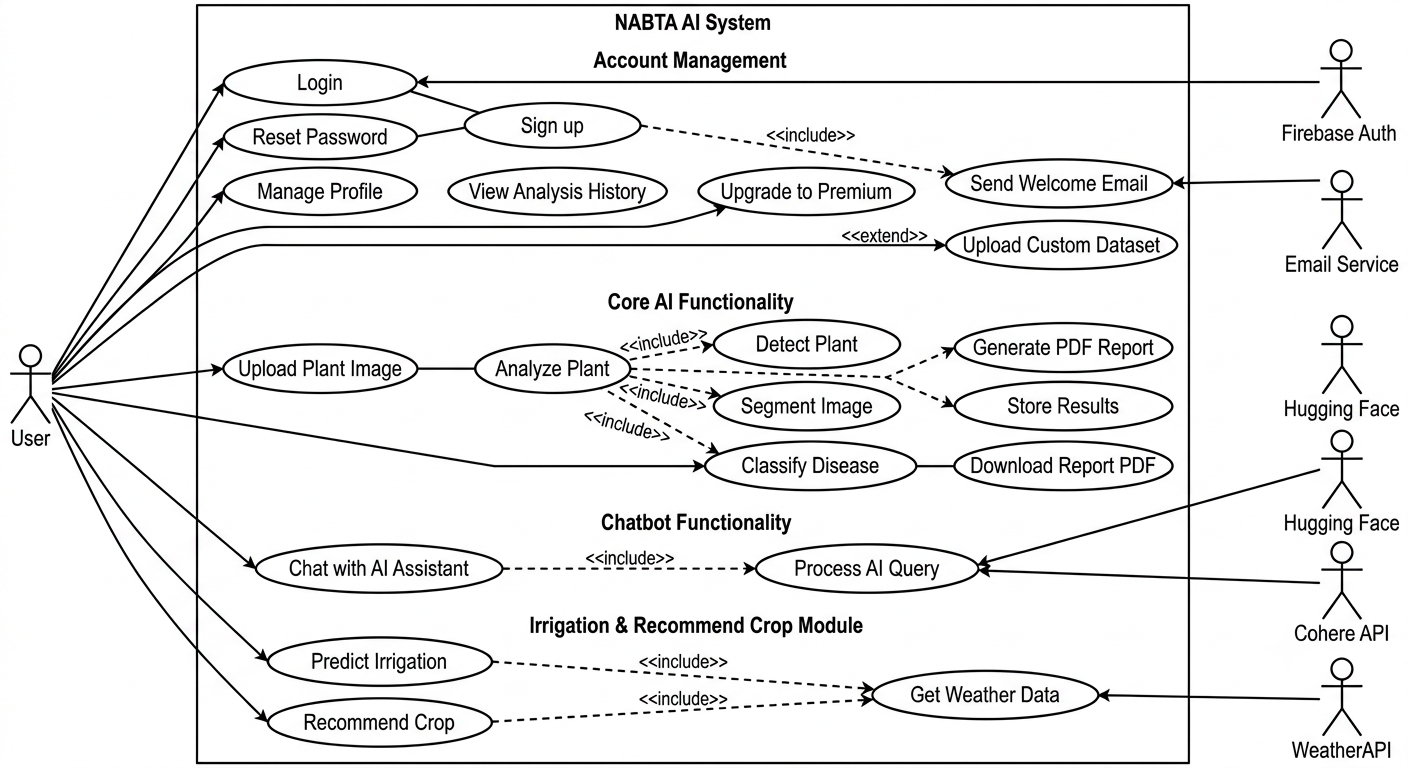
\includegraphics[width=\textwidth]{assets/diagrams/use_case_diagram.png}
\caption{Use Case Diagram of the NABTA Platform}
\label{fig:use_case}
\end{figure}

The system primarily interacts with two categories of actors:

\begin{itemize}
\item \textbf{User}, who utilizes the intelligent agricultural services.
\item \textbf{Administrator}, who manages system resources and user accounts.
\end{itemize}

External services including Firebase Authentication, Cohere API, Hugging Face, Weather API, and Email Services cooperate with the system to provide authentication, artificial intelligence inference, weather information, and notification services.

The User actor can perform the following operations:

\begin{itemize}
\item Register and authenticate.
\item Upload plant images.
\item Analyze plant diseases.
\item View disease reports.
\item Generate PDF reports.
\item Communicate with the AI Assistant.
\item Obtain crop recommendations.
\item Receive irrigation recommendations.
\item Browse previous analysis records.
\item View analytical dashboards.
\item Manage personal profile information.
\end{itemize}

The Administrator possesses additional privileges, including managing users, monitoring system status, maintaining agricultural datasets, and supervising platform resources.

The use case diagram demonstrates that all intelligent services are accessed through a unified interface while authentication and authorization mechanisms ensure secure access to protected resources.

%==============================================================================
\section{Activity Diagram}
\label{sec:activity_diagram}

The Activity Diagram illustrates the sequence of operations performed during the plant disease diagnosis process. It describes how user interactions trigger successive software components until the final diagnosis is produced.

Figure~\ref{fig:activity_diagram} presents the activity diagram of the proposed system.

\begin{figure}[H]
\centering
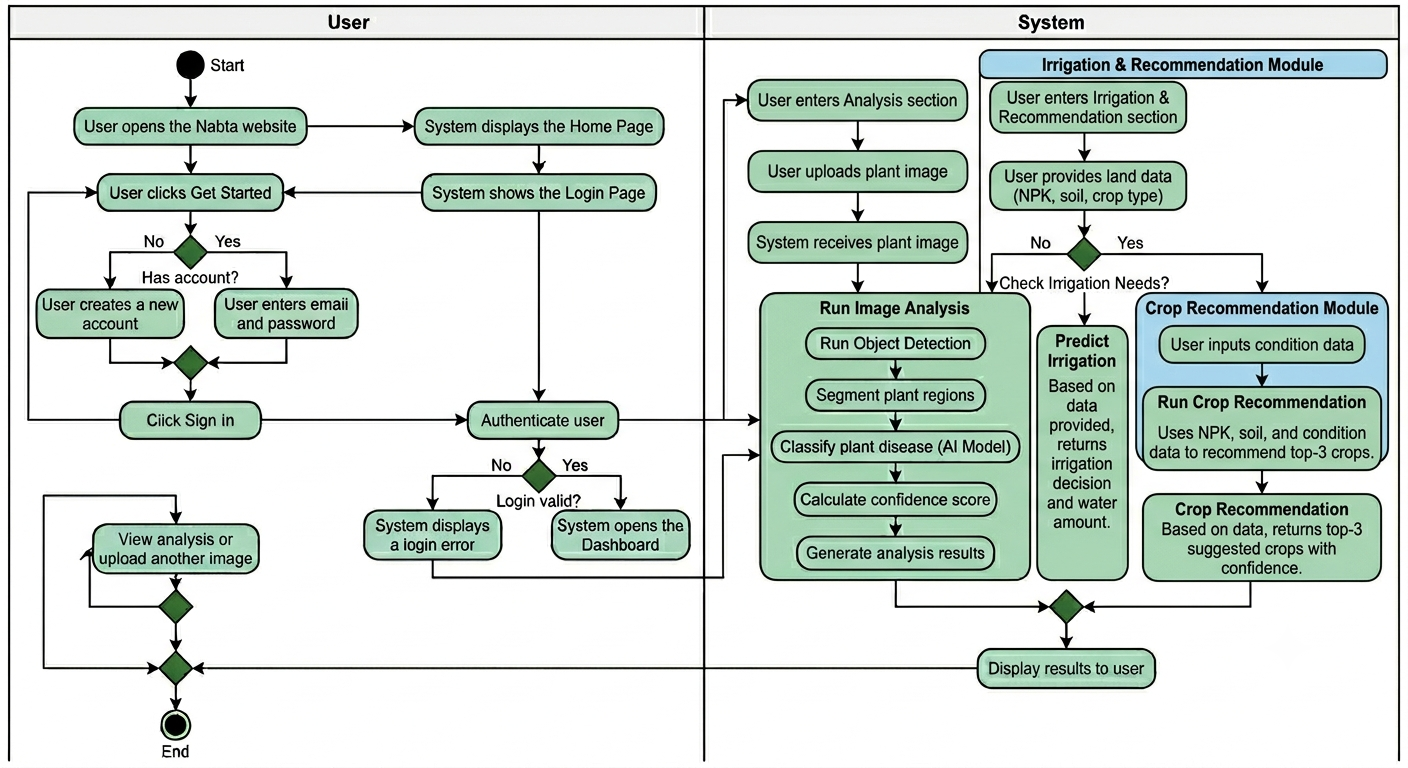
\includegraphics[width=.95\textwidth]{assets/diagrams/activity_diagram.png}
\caption{Activity Diagram of the Plant Disease Diagnosis Process}
\label{fig:activity_diagram}
\end{figure}

The workflow begins when the user uploads a plant image through the web interface. The backend validates the uploaded image before forwarding it to the artificial intelligence pipeline.

The YOLOv8x detector first localizes the infected leaf region. The cropped image is then processed by the U-Net segmentation model to isolate the leaf from the background. The segmented image is subsequently classified using the CNN model, which predicts one of the supported plant disease classes.

Grad-CAM generates an explainability heatmap and estimates disease severity. Finally, the diagnosis report is generated, stored in Firebase Cloud Firestore, and presented to the user through the frontend interface.

This sequential workflow minimizes unnecessary computations while ensuring that every stage receives optimized input from the previous model.

%==============================================================================
\section{Sequence Diagram}
\label{sec:sequence_diagram}

The Sequence Diagram describes the interactions among the user, frontend application, backend services, artificial intelligence models, and cloud infrastructure during a typical disease diagnosis session.

Figure~\ref{fig:sequence_diagram} illustrates these interactions.

\begin{figure}[H]
\centering
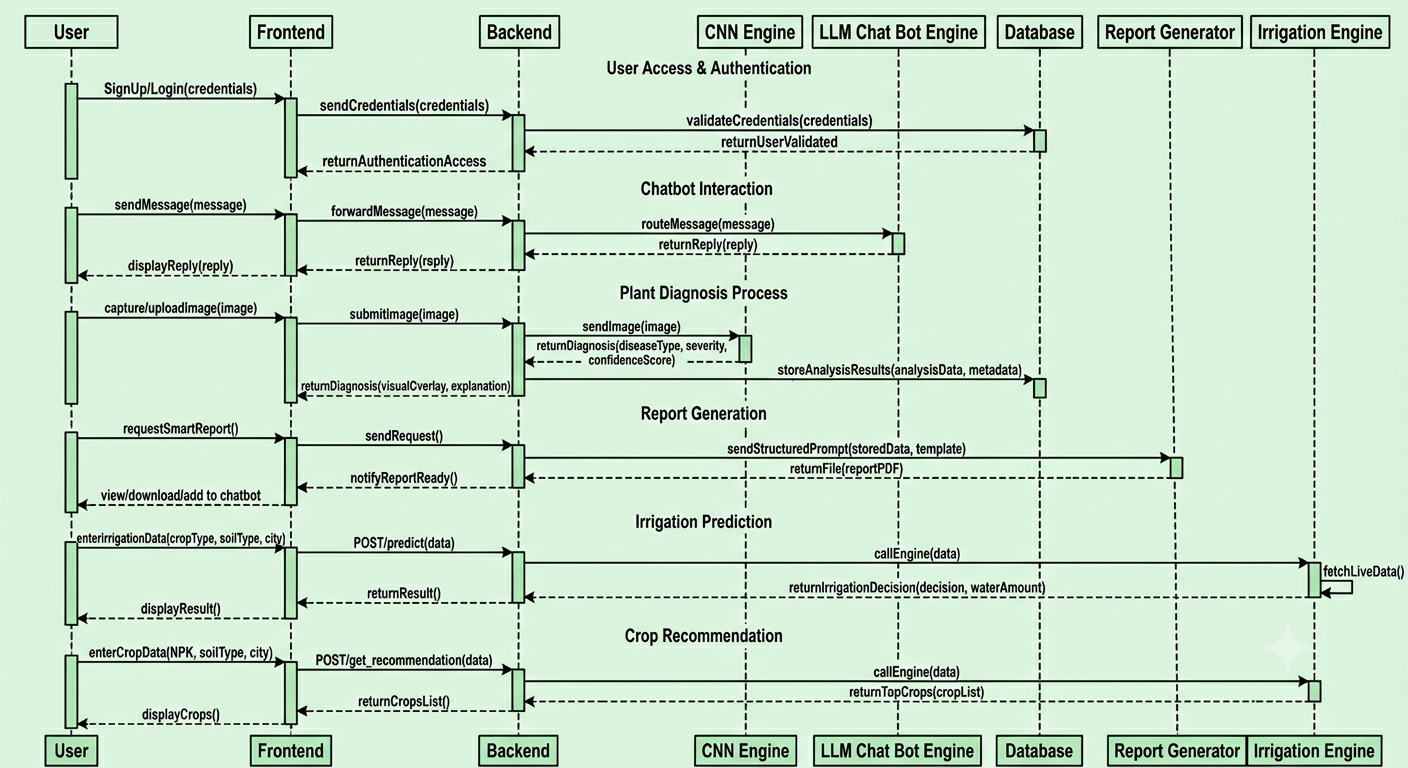
\includegraphics[width=\textwidth]{assets/diagrams/sequence_diagram.png}
\caption{Sequence Diagram of the NABTA Platform}
\label{fig:sequence_diagram}
\end{figure}

The interaction begins when the user uploads a plant image through the React.js frontend. The frontend transmits the image to the FastAPI backend, which performs validation before initiating the AI pipeline.

The backend sequentially invokes the YOLOv8x detection model, the U-Net segmentation model, and the CNN classifier. Once classification is completed, Grad-CAM generates the explainability visualization and disease severity estimation.

The generated diagnosis is stored in Cloud Firestore, while optional PDF reports are produced upon user request.

When agricultural consultation is requested, the backend retrieves relevant knowledge through the Retrieval-Augmented Generation (RAG) pipeline before forwarding the enriched prompt to the Cohere Large Language Model.

Finally, all generated outputs are returned to the frontend and displayed through the user interface.

%==============================================================================
\section{Class Diagram}
\label{sec:class_diagram}

The object-oriented structure of the software system is represented using the UML Class Diagram shown in Figure~\ref{fig:class_diagram}.

\begin{figure}[H]
\centering
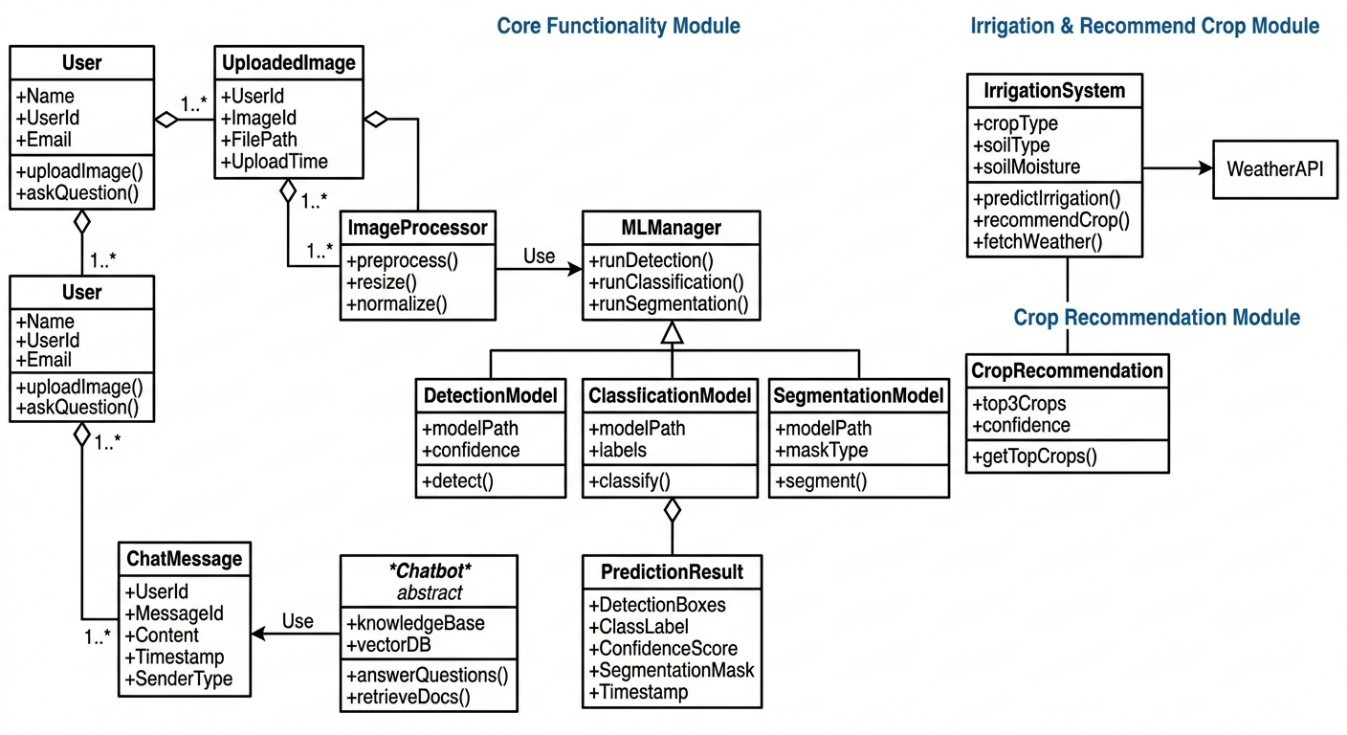
\includegraphics[width=\textwidth]{assets/diagrams/class_diagram.png}
\caption{Class Diagram of the NABTA Platform}
\label{fig:class_diagram}
\end{figure}

The system is composed of multiple logical classes responsible for user management, plant analysis, disease reports, chatbot interaction, crop recommendation, irrigation prediction, and report generation.

Relationships between these classes improve modularity while supporting future extensibility and maintainability.

Each software component encapsulates its own responsibilities, reducing coupling and improving software quality.

%==============================================================================
\section{Entity Relationship Diagram}
\label{sec:erd}

The persistent data used by the NABTA platform are stored in Google Cloud Firestore. Although Firestore is a NoSQL document-oriented database, the logical relationships between the major entities can still be represented using an Entity Relationship Diagram (ERD).

Figure~\ref{fig:erd} illustrates the logical data model adopted in the proposed platform.

\begin{figure}[H]
\centering
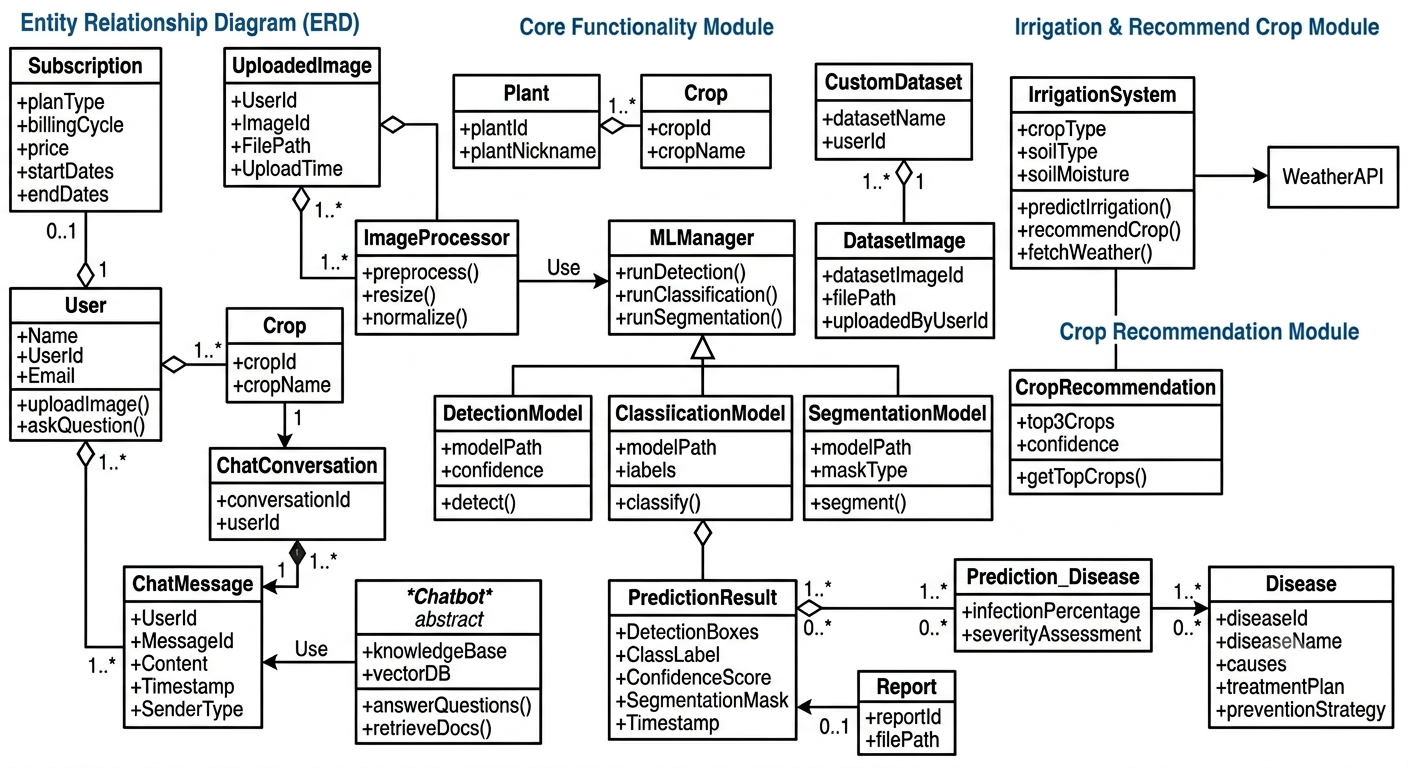
\includegraphics[width=.95\textwidth]{assets/diagrams/entity_relationship_diagram.png}
\caption{Entity Relationship Diagram of the NABTA Platform}
\label{fig:erd}
\end{figure}

The database is organized around several primary entities that store user information, plant disease analyses, chatbot conversations, recommendation records, and generated reports.

The main entities include:

\begin{itemize}

\item Users

\item Plant Analysis

\item Disease Reports

\item Chat History

\item Crop Recommendations

\item Irrigation Records

\item PDF Reports

\item Custom Dataset

\end{itemize}

Each authenticated user may own multiple disease analyses, recommendation records, chatbot conversations, and generated reports, allowing the platform to maintain a complete history of agricultural activities.

The document-oriented design of Cloud Firestore provides high scalability, low latency, and seamless synchronization with the frontend application.

%==============================================================================
\section{Database Design}
\label{sec:database_design}

The NABTA platform utilizes Firebase Cloud Firestore as its primary cloud database. Firestore stores information as collections of JSON-like documents, enabling flexible schema evolution while supporting real-time synchronization.

The major collections implemented in the platform are summarized in Table~\ref{tab:firestore_collections}.

\begin{table}[H]
\centering
\caption{Firestore Collections}
\label{tab:firestore_collections}
\renewcommand{\arraystretch}{1.35}

\begin{tabularx}{\textwidth}{>{\raggedright\arraybackslash}p{4cm}X}

\toprule

\textbf{Collection} &
\textbf{Description}

\\

\midrule

Users &
Stores user account information, authentication identifiers, profile details, and subscription information.

\\

PlantAnalysis &
Stores uploaded images, disease predictions, confidence scores, Grad-CAM visualizations, and disease severity estimations.

\\

DiseaseReports &
Stores generated disease diagnosis reports and treatment recommendations.

\\

ChatHistory &
Stores conversations between users and the AI agricultural assistant.

\\

CropRecommendations &
Stores crop recommendation requests together with predicted crops and confidence values.

\\

IrrigationRecords &
Stores irrigation prediction requests, irrigation decisions, and estimated crop water requirements.

\\

PDFReports &
Stores metadata associated with generated PDF reports.

\\

CustomDataset &
Stores administrator-managed agricultural knowledge and user-defined records.

\\

\bottomrule

\end{tabularx}

\end{table}

Each document is uniquely identified using Firebase-generated document identifiers. Relationships between documents are maintained using user identifiers and analysis identifiers, enabling efficient retrieval of historical records without introducing unnecessary data duplication.

The adopted database design supports horizontal scalability while maintaining high availability and low response latency.

%==============================================================================
\subsection{Database Relationships}

Although Firestore is a document-oriented database, logical relationships exist between the stored collections.

A single user may perform multiple plant analyses, generate multiple PDF reports, communicate with the AI assistant several times, and request both irrigation and crop recommendations.

The principal relationships are summarized below:

\begin{itemize}

\item One User $\rightarrow$ Many Plant Analysis Records

\item One User $\rightarrow$ Many Disease Reports

\item One User $\rightarrow$ Many Chat Conversations

\item One User $\rightarrow$ Many Crop Recommendations

\item One User $\rightarrow$ Many Irrigation Records

\item One User $\rightarrow$ Many PDF Reports

\end{itemize}

This logical organization simplifies historical record retrieval while maintaining data consistency throughout the platform.

%==============================================================================
\section{Component Diagram}
\label{sec:component_diagram}

The Component Diagram illustrates the modular organization of the NABTA platform and the interactions among its major software components.

Figure~\ref{fig:component_diagram} presents the component architecture adopted in the proposed system.

\begin{figure}[H]
\centering
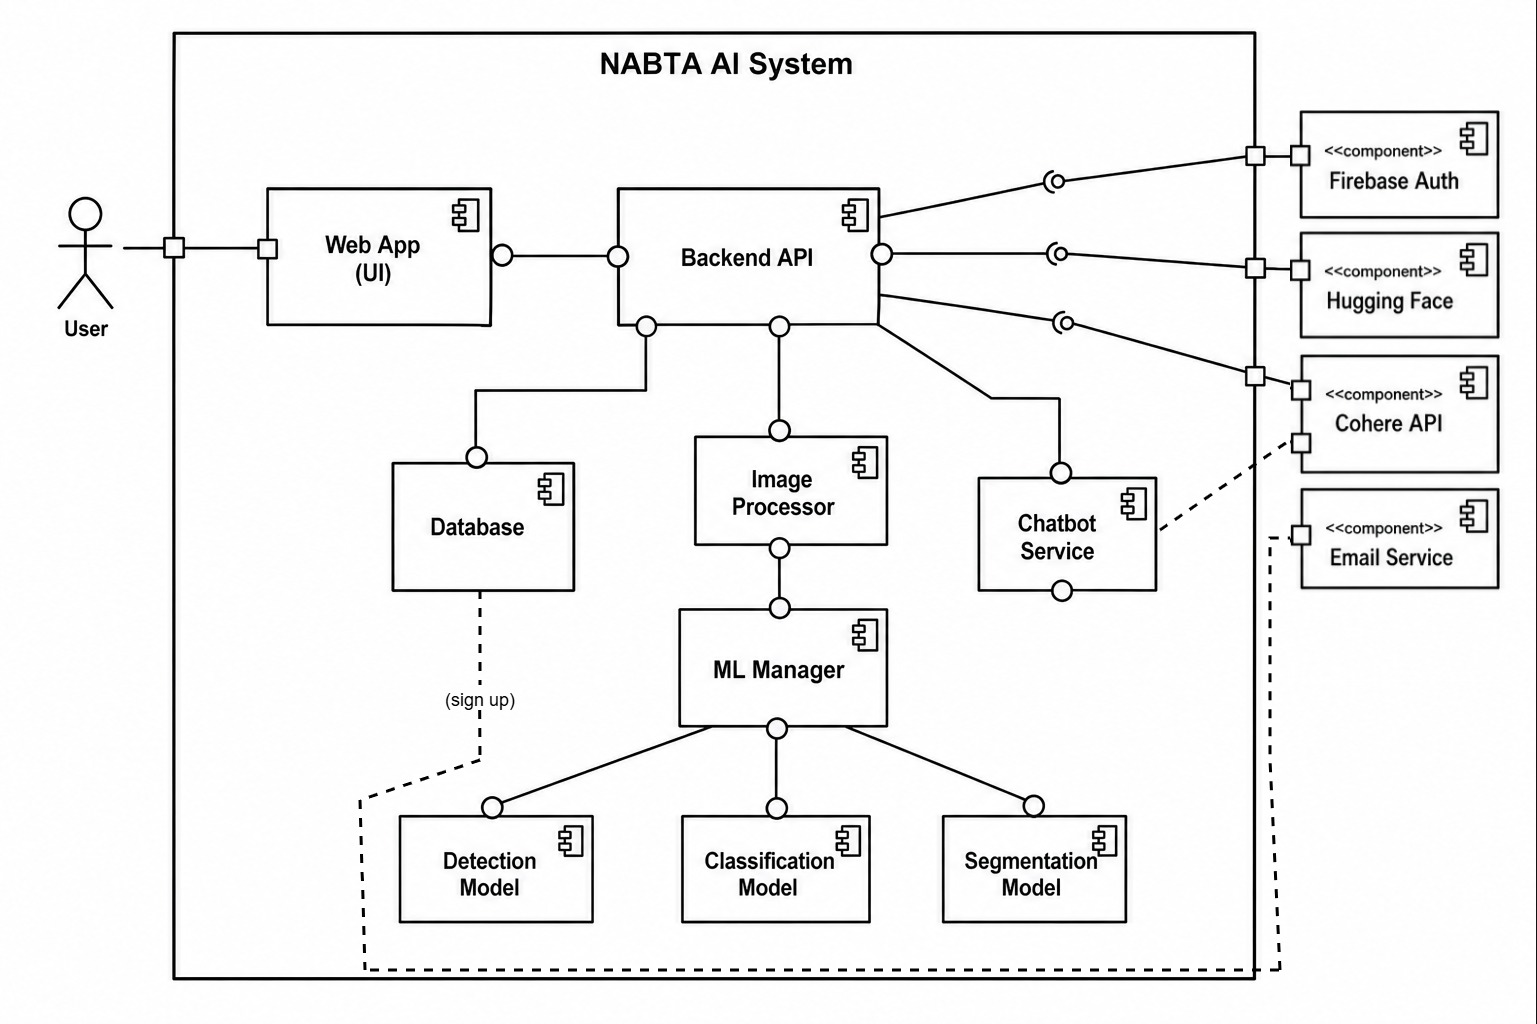
\includegraphics[width=\textwidth]{assets/diagrams/component_diagram.jpeg}
\caption{Component Diagram of the NABTA Platform}
\label{fig:component_diagram}
\end{figure}

The platform consists of several independent but interconnected software components, each responsible for a specific functionality.

The major components include:

\begin{itemize}

\item React.js Frontend

\item FastAPI Backend

\item Authentication Service

\item Plant Disease Analysis Service

\item YOLOv8x Detection Service

\item U-Net Segmentation Service

\item CNN Classification Service

\item Grad-CAM Explainability Service

\item Crop Recommendation Service

\item Irrigation Recommendation Service

\item AI Assistant Service

\item PDF Report Generator

\item Firebase Cloud Services

\item Cloud Firestore Database

\end{itemize}

The modular architecture allows every component to operate independently while communicating through RESTful APIs. Such separation simplifies future maintenance, testing, and deployment.

%==============================================================================
\section{Deployment Diagram}
\label{sec:deployment}

The Deployment Diagram illustrates how software components are distributed across cloud infrastructure and client devices.

Figure~\ref{fig:deployment_diagram} presents the deployment architecture of NABTA.

\begin{figure}[H]
\centering
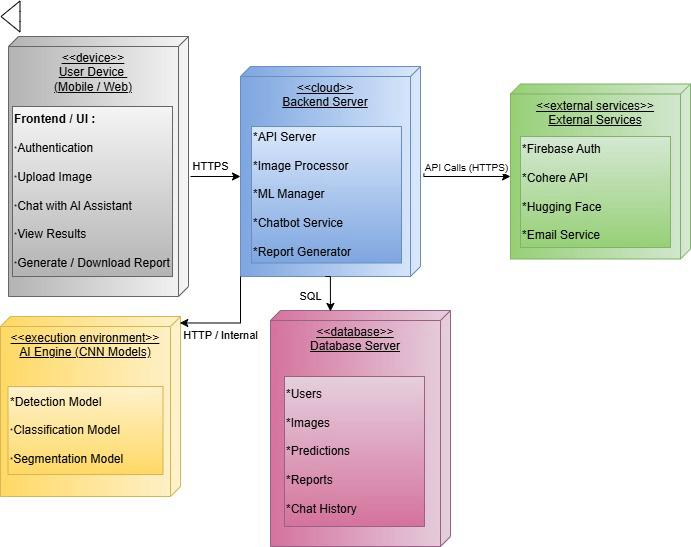
\includegraphics[width=\textwidth]{assets/diagrams/deployment_diagram.jpeg}
\caption{Deployment Diagram of the NABTA Platform}
\label{fig:deployment_diagram}
\end{figure}

The deployment architecture consists of four major nodes:

\begin{enumerate}

\item Client Device

\item Frontend Server

\item Backend Server

\item Cloud Services

\end{enumerate}

Users access the platform through modern web browsers. The React.js application communicates with the FastAPI backend using HTTPS requests.

The backend performs AI inference by invoking the deployed computer vision and machine learning models. Firebase Authentication verifies user identities, while Cloud Firestore stores persistent application data.

The Cohere API is responsible for generating intelligent conversational responses through the Retrieval-Augmented Generation (RAG) pipeline, whereas Hugging Face hosts the deployed deep learning inference services.

This deployment strategy provides scalability, security, and efficient resource utilization.

%==============================================================================
\section{REST API Design}
\label{sec:api_design}

Communication between the frontend application and backend services is performed through RESTful APIs implemented using FastAPI.

Each API endpoint performs a dedicated task while exchanging data in JSON format.

Table~\ref{tab:api_endpoints} summarizes the principal REST API endpoints implemented in the NABTA platform.

\begin{table}[H]
\centering
\caption{Main REST API Endpoints}
\label{tab:api_endpoints}
\renewcommand{\arraystretch}{1.35}

\begin{tabularx}{\textwidth}{>{\raggedright\arraybackslash}p{4cm}>{\raggedright\arraybackslash}p{3cm}X}

\toprule

\textbf{Endpoint} &
\textbf{Method} &
\textbf{Purpose}

\\

\midrule

/api/detect &
POST &
Detect infected leaf using YOLOv8x.

\\

/api/segment &
POST &
Generate the leaf segmentation mask.

\\

/api/classify &
POST &
Predict plant species and disease class.

\\

/api/analyze &
POST &
Execute the complete AI analysis pipeline.

\\

/api/chat &
POST &
Generate AI agricultural consultation.

\\

/api/crop-recommendation &
POST &
Recommend suitable crops.

\\

/api/irrigation &
POST &
Predict irrigation decision.

\\

/api/water-requirement &
POST &
Estimate crop water requirement.

\\

/api/report &
POST &
Generate PDF disease reports.

\\

/api/history &
GET &
Retrieve previous analysis records.

\\

/api/profile &
GET &
Retrieve user profile information.

\\

\bottomrule

\end{tabularx}

\end{table}

The REST architecture enables loose coupling between the frontend and backend while allowing individual services to evolve independently. FastAPI automatically generates OpenAPI documentation, simplifying API testing and future integration with external applications.

%==============================================================================
\section{Security Architecture}
\label{sec:security}

Security represents one of the fundamental design considerations of the NABTA platform. Since the system processes user accounts, uploaded plant images, historical records, and artificial intelligence services, multiple security mechanisms were incorporated throughout the system architecture.

The proposed security framework consists of several complementary layers that collectively protect user information, backend services, and cloud resources.

\subsection{Authentication and Authorization}

User authentication is managed through Firebase Authentication using secure email and password credentials.

After successful authentication, Firebase generates a JSON Web Token (JWT) that accompanies every protected request sent to the backend. The FastAPI server validates this token before granting access to secured endpoints, ensuring that only authenticated users can utilize protected platform services.

Role-based authorization is also supported, allowing administrators to access management functions while restricting regular users to their own resources.

\subsection{Secure API Communication}

All communication between the frontend and backend is performed through HTTPS using encrypted TLS connections.

The backend validates every incoming request before processing, including:

\begin{itemize}

\item Authentication token verification.

\item Uploaded image validation.

\item Input parameter validation.

\item File type verification.

\item Request size limitation.

\end{itemize}

These validation mechanisms reduce the risk of malformed requests and unauthorized access.

\subsection{API Key Protection}

Sensitive credentials such as the Cohere API key, Firebase configuration, and external service tokens are never embedded directly within the frontend application.

Instead, all confidential information is stored securely using environment variables on the backend server. This prevents accidental exposure of credentials while simplifying deployment across different environments.

\subsection{Cloud Security}

Firebase Authentication and Cloud Firestore implement multiple built-in security mechanisms including encrypted communication, access control rules, and user-based authorization.

Firestore security rules ensure that users can access only their own analysis records, generated reports, and chatbot conversations.

These cloud-level protections significantly improve overall platform security without increasing implementation complexity.

%==============================================================================
\section{Design Principles}
\label{sec:design_principles}

Several software engineering principles guided the design of the proposed NABTA platform.

\begin{itemize}

\item \textbf{Modularity}

Each intelligent component operates as an independent service with clearly defined responsibilities.

\item \textbf{Scalability}

The architecture allows additional artificial intelligence models or cloud services to be integrated without major structural modifications.

\item \textbf{Maintainability}

Independent software modules simplify debugging, testing, maintenance, and future system upgrades.

\item \textbf{Reusability}

Reusable frontend components and backend APIs reduce software duplication while improving development efficiency.

\item \textbf{Loose Coupling}

RESTful communication minimizes dependencies between the frontend, backend, artificial intelligence models, and cloud services.

\item \textbf{High Cohesion}

Each module performs one primary responsibility, resulting in improved software quality and readability.

\end{itemize}

Applying these principles resulted in a flexible architecture capable of supporting future expansion while maintaining high software quality.

%==============================================================================
\section{Design Decisions}
\label{sec:design_decisions}

Several important architectural decisions were made during the development of NABTA.

React.js was selected for frontend development because of its component-based architecture, excellent performance, and extensive ecosystem.

FastAPI was adopted as the backend framework due to its asynchronous request handling, automatic API documentation, and high inference performance.

YOLOv8x was selected for object detection because it achieved superior localization accuracy compared with smaller YOLO variants.

U-Net with an EfficientNet-B0 encoder was chosen for semantic segmentation because it provides an excellent balance between segmentation accuracy and computational efficiency.

The disease classification module employs a custom CNN specifically designed for large-scale plant disease recognition across 102 classes.

Random Forest was selected for crop recommendation and irrigation prediction because it demonstrated strong predictive performance, robustness against overfitting, and excellent generalization capability.

Firebase provides authentication, cloud storage, and backend services, while Cohere and Retrieval-Augmented Generation enable intelligent agricultural consultation with improved factual consistency.

Collectively, these design decisions resulted in a scalable, maintainable, and production-ready smart agriculture platform.

%==============================================================================
\section{Chapter Summary}
\label{sec:chapter4_summary}

This chapter presented the complete architectural design of the NABTA smart agriculture platform.

The overall system architecture, execution workflow, UML diagrams, database structure, deployment strategy, REST API architecture, and security mechanisms were discussed in detail. Furthermore, the chapter described the software engineering principles and architectural decisions that guided the implementation of the platform.

The proposed design provides a modular, scalable, secure, and maintainable foundation that supports the integration of multiple artificial intelligence models within a unified web-based application.

The following chapter presents the implementation details of the developed system, including the frontend interfaces, backend services, artificial intelligence integration, cloud deployment, and user interaction.
